%%%%%%%%%%%%%%%%%%%%%%%%%%%%%%%%%%%%%%%%%%%%%%%%%%%%%%%%%%%%%%%%%%%%%%%%%%%%%%%%%%%%%%%%%%%%%%%%%%%%
% ==================================================================================================
% --------------------------------------------------------------------------------------------------
\chapter{Implementation}
This appendix contains implementation details.
%%%%%%%%%%%%%%%%%%%%%%%%%%%%%%%%%%%%%%%%%%%%%%%%%%%%%%%%%%%%%%%%%%%%%%%%%%%%%%%%%%%%%%%%%%%%%%%%%%%%
\section{Computing}
All computation in the current work was performed using the following workstation and software:
\begin{itemize}[topsep=0pt,itemsep=-6pt]
  \item \textbf{CPU:} Intel Core i7-6700K 4.00 GHz
  \item \textbf{RAM:} 16.0 GB DDR4
  \item \textbf{GPU:} NVIDIA GeForce GTX 980 Ti
  \item \textbf{OS:} Windows 10 Pro
  \item \textbf{Code:} MATLAB R2011a
\end{itemize}
%%%%%%%%%%%%%%%%%%%%%%%%%%%%%%%%%%%%%%%%%%%%%%%%%%%%%%%%%%%%%%%%%%%%%%%%%%%%%%%%%%%%%%%%%%%%%%%%%%%%
\section{Parallel Model Fitting}\label{s:parallelfit}
Speed of model fitting is a significant factor during development, particularly considering optimization of so-called hyperparameters. Faster training yields more model iterations, which inevitably bear improvements. While the estimation procedure outlined in \S\ \ref{ss:modelfitting} must be repeated for all standardized voxels in the brain mask, it is possible to do this in parallel, since every estimation is independent. To do so, the training data must first be vectorized with respect to spatial location $x$, and matrix operations expanded explicitly to accommodate the new dimension.
\par
% __JK__ does this (below) belong in the appendix?
% __JK__ (yes!)
To begin, the standardized training data from all subjects -- features $\tilde{\bm{\Y}}(x)$, with $\tilde{\Y}^{\et0}=1$, and labels $\C(x)$ -- are sampled from nonzero locations in the brain mask $M(x)$. These data are stored in two matrices $\x{Y}$ and $\x{C}$, with dimensions $[V,N,K+1]$ and $[V,N,1]$, respectively, where $V$ is the total number of nonzero voxels in the brain mask, $N$ is the number of subjects, and $K$ is the number of features. A similar matrix is constructed for the initial parameters $\bb^{(0)}(x)$, denoted $\x{B}^{(0)}$, with dimensions $[V,1,K+1]$. Let $\x{Y}_n^k$ denote the vector of data from all voxels for the $k$\ss{th} feature from the $n$\ss{th} subject, and so on for $\x{C}$ and $\x{B}$.
\par
In order to simplify subsequent calculations, the feature data are rectified according to the class labels, before the first iteration, as in
\begin{equation}
\x{Y}_n^k =
\begin{cases}
+\x{Y}_n^k, & \x{C}_n \ge 0.5\\
-\x{Y}_n^k, & \x{C}_n <  0.5\\
\end{cases},\qquad\forall\et k \in \{1,\dots,K\}.
\end{equation}
Next, for a given iteration $t$, the following vector-compatible expansions of Equations (\ref{eq:llgradient}), (\ref{eq:llhessian}), and (\ref{eq:newtonmap}) yield the desired update matrix $\Delta\x{B}^{(t)}$. These calculations are performed in \nameref{m:logreg.m}.
Regarding notation:
1) the iteration index ${}^{(t)}$ is omitted for clarity,
2) element-wise multiplication is denoted by $\circ$, and
3) the variable $K$ is now defined as $1$, since this is essential to the simplification.
\begin{align}
\x{S} &= \frac{1}{1+e^{\et\eta}},\qquad \eta = \x{B}^0 + \left(\x{B}^1\ep\x{Y}^1\right)\\
\x{A} &= \x{S}\ep\left(1-\x{S}\right)\\
\x{G} &= \nabla_{\x{B}}\L - \lambda\x{B} \nonumber \\
&= \left[\begin{array}{c}
\x{G}^1 \\ \x{G}^2
\end{array}\right] \nonumber \\
&= \left[\begin{array}{c}
\sum_{n=1}^{N}\left( \x{Y}_n^1\circ\x{S} \right) \\
\sum_{n=1}^{N}\left( \x{Y}_n^2\circ\x{S} \right)
\end{array}\right] - \lambda\left[\begin{array}{c} \x{B}^1 \\ \x{B}^2\end{array}\right]\\
\x{H} &= \nabla_{\x{B}}^2\L -\lambda\x{I} \nonumber \\
&= \left[\begin{array}{cc}
\x{H}^{1,1} & \x{H}^{1,2} \\ \x{H}^{2,1} & \x{H}^{2,2}
\end{array}\right] \nonumber \\
&= \left[\begin{array}{cc}
\sum_{n=1}^{N}\left( \x{A}\circ\x{Y}_n^1\circ\x{Y}_n^1 \right) & 
\sum_{n=1}^{N}\left( \x{A}\circ\x{Y}_n^2\circ\x{Y}_n^1 \right) \\
\sum_{n=1}^{N}\left( \x{A}\circ\x{Y}_n^1\circ\x{Y}_n^2 \right) & 
\sum_{n=1}^{N}\left( \x{A}\circ\x{Y}_n^2\circ\x{Y}_n^2 \right)
\end{array}\right] - \lambda\left[\begin{array}{cc} 1 & \\ & 1\end{array}\right]\\
\x{D} &= \det{\x{H}} \nonumber \\
&= \left(\x{H}^{1,1}\circ\x{H}^{2,2}\right) - \left(\x{H}^{1,2}\circ\x{H}^{2,1}\right) \\
\Delta\x{B} &= -\x{H}^{-1}\x{G} \nonumber \\
&= \dfrac{1}{\x{D}} \left[\begin{array}{cc}
\left(\x{H}^{2,2}\circ\x{G}^{1} - \x{H}^{2,1}\circ\x{G}^{2} \right) & 
\left(\x{H}^{1,2}\circ\x{G}^{2} - \x{H}^{1,1}\circ\x{G}^{1} \right)
\end{array}\right]^{T}
\end{align}
%%%%%%%%%%%%%%%%%%%%%%%%%%%%%%%%%%%%%%%%%%%%%%%%%%%%%%%%%%%%%%%%%%%%%%%%%%%%%%%%%%%%%%%%%%%%%%%%%%%%
\section{Manual Segmentations}
It was necessary to create and edit a small number of binary segmentation masks during this work. To do this, the Editor module from the 3D Slicer imaging platform \cite{Fedorov2012} was used\footnote{3D Slicer Editor tool documentation is available here: \hreftt{https://www.slicer.org/wiki/Documentation/4.6/Modules/Editor}.}, including the Wand, Paint, and Erase functions. Figure \ref{fig:m08-rev-slicer} shows the user interface during a lesion segmentation.
\begin{figure}[h]
  \centering
  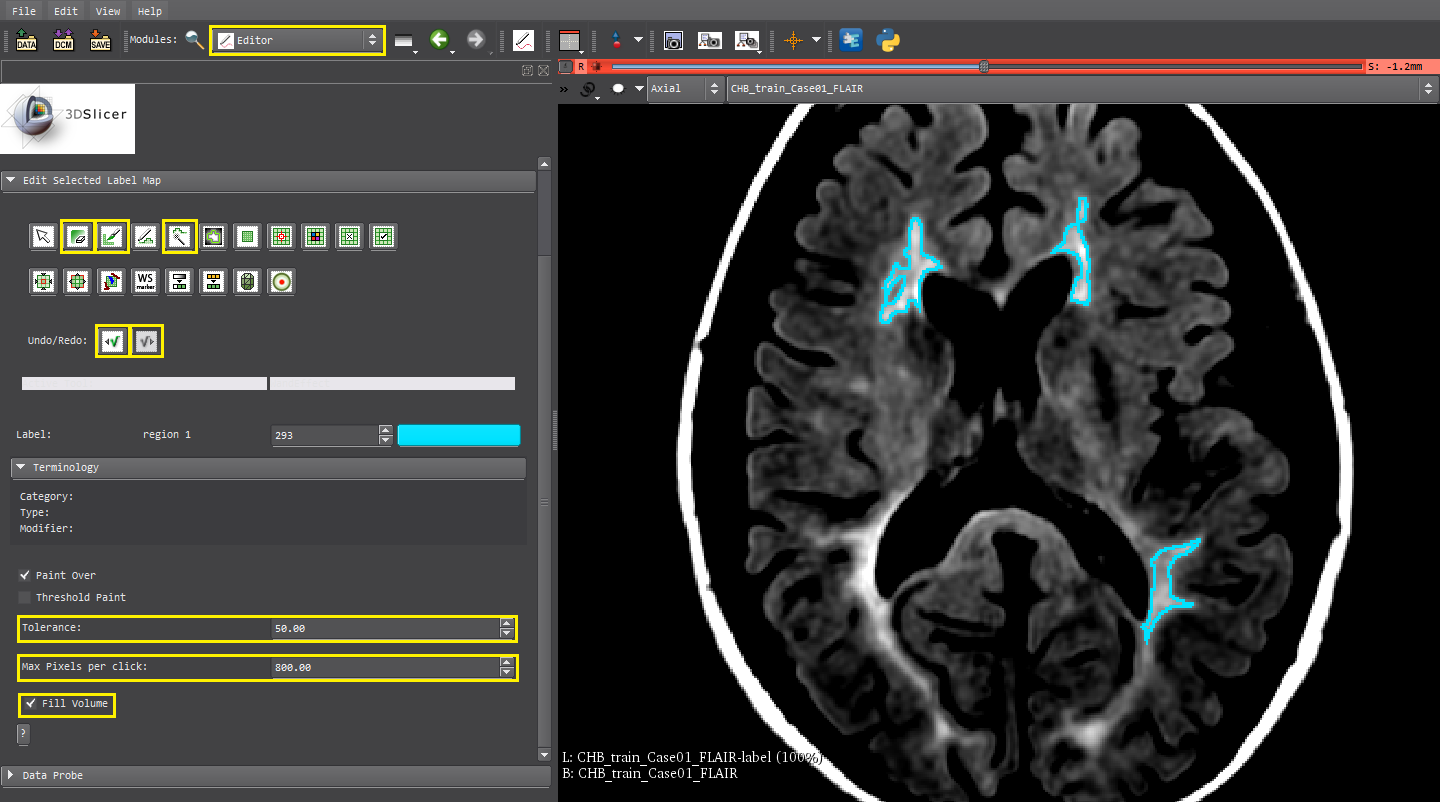
\includegraphics[width=\textwidth]{m08rev-slicer.png}
  \caption{3D Slicer user interface for performing in-house manual segmentations and revisions. The tools used are highlighted in yellow, while the segmentation (in-progress) is shown in blue.}
  \label{fig:m08-rev-slicer}
\end{figure}
% ==================================================================================================
\subsection{MS 2008 WMH Masks}\label{ss:m08-rev}
Since the reported performance of an automatic segmentation algorithm depends on the manual segmentations to which it is compared, it is important to obtain good manual segmentations. Unfortunately, the original manuals in the MS 2008 Segmentation Challenge contained obvious artifacts and inconsistencies, as shown at left in Figure \ref{fig:m08-rev}. Therefore, it was deemed necessary to redo these manuals. The resulting revisions are shown at right in Figure \ref{fig:m08-rev}.
\begin{figure}
  \centering
  \begin{minipage}{6cm}
    \begin{subfigure}{\textwidth}
      \centering\subcaption{Original}\label{fig:m08-rev-o}
      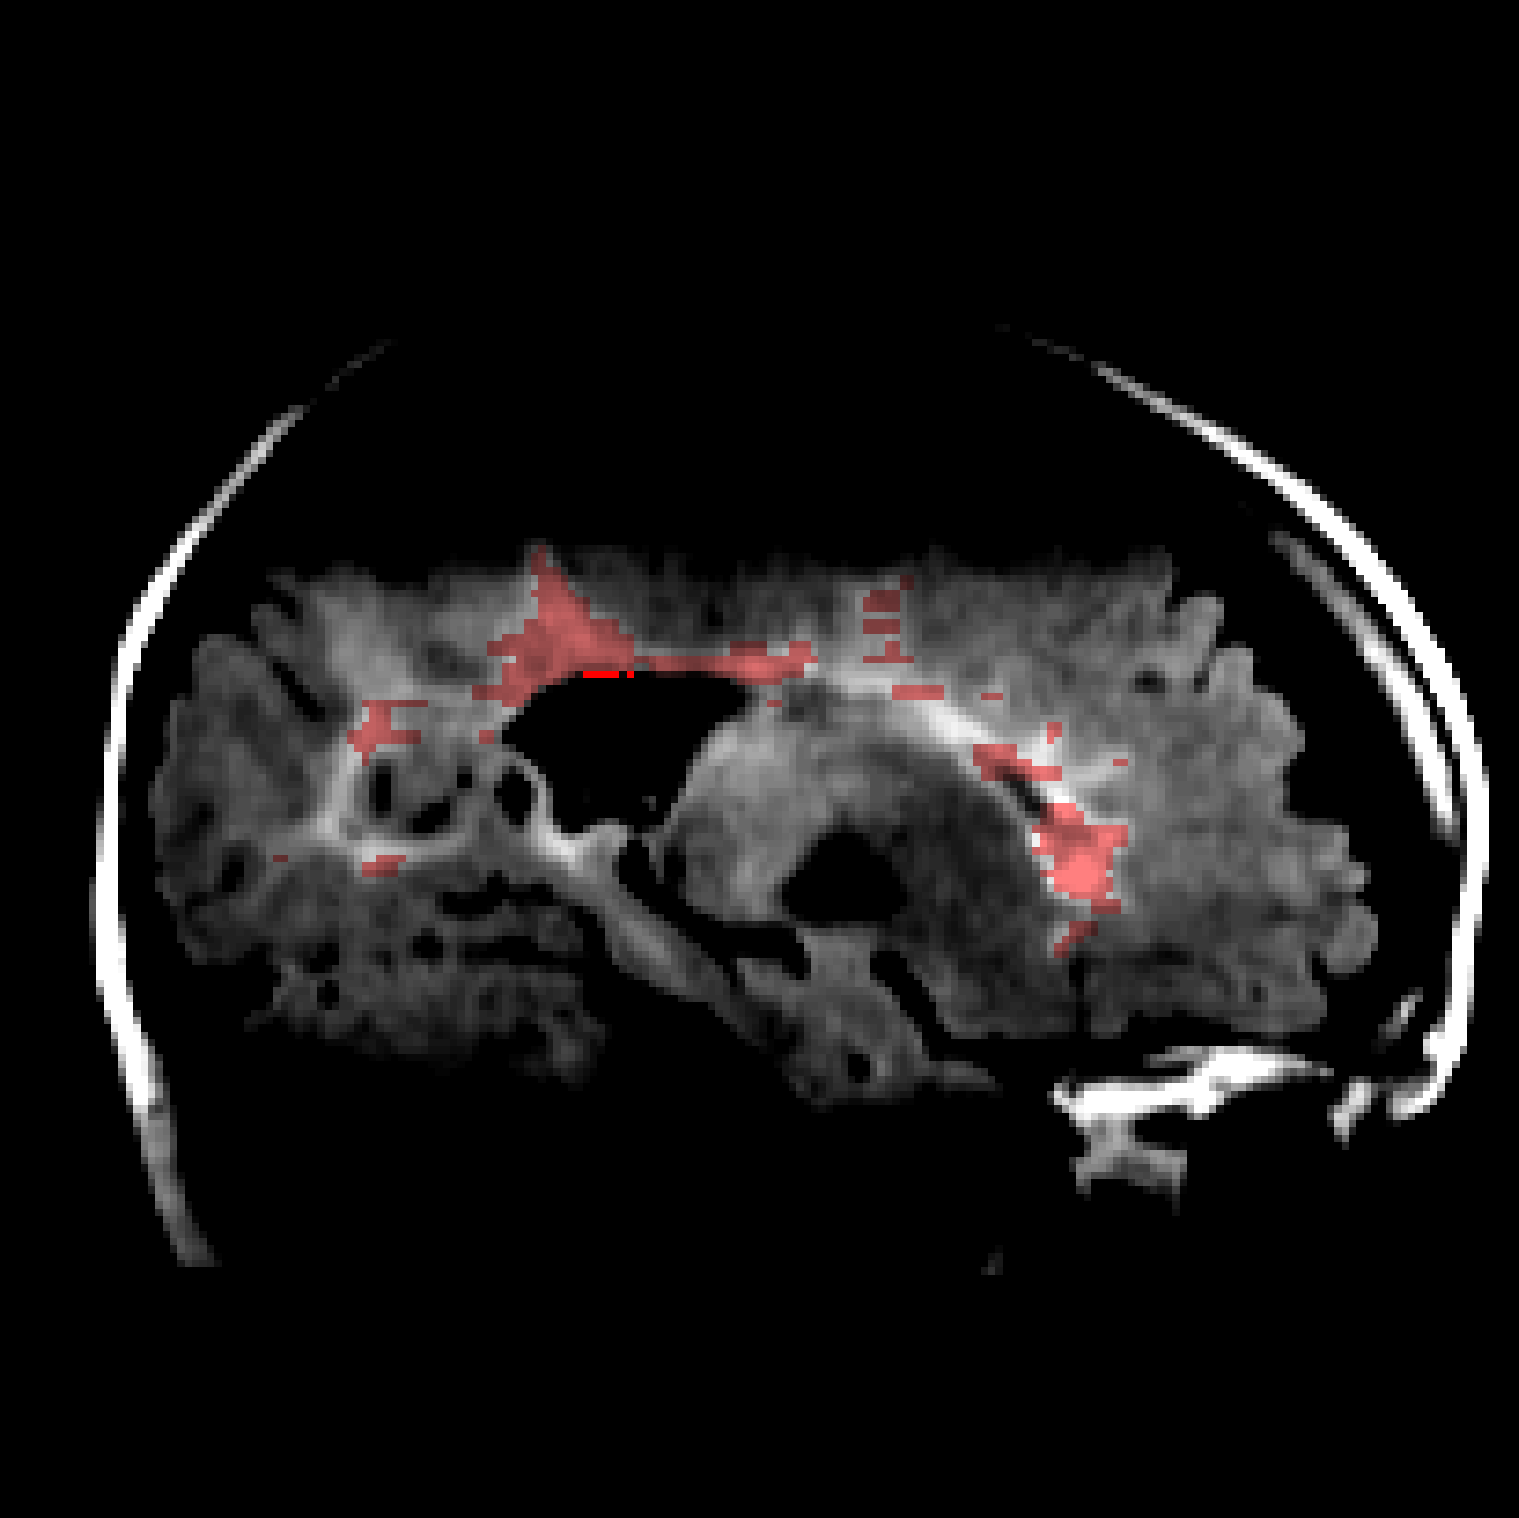
\includegraphics[height=6cm]{m08rev-01-d2-z146-o}\\[0.2em]
      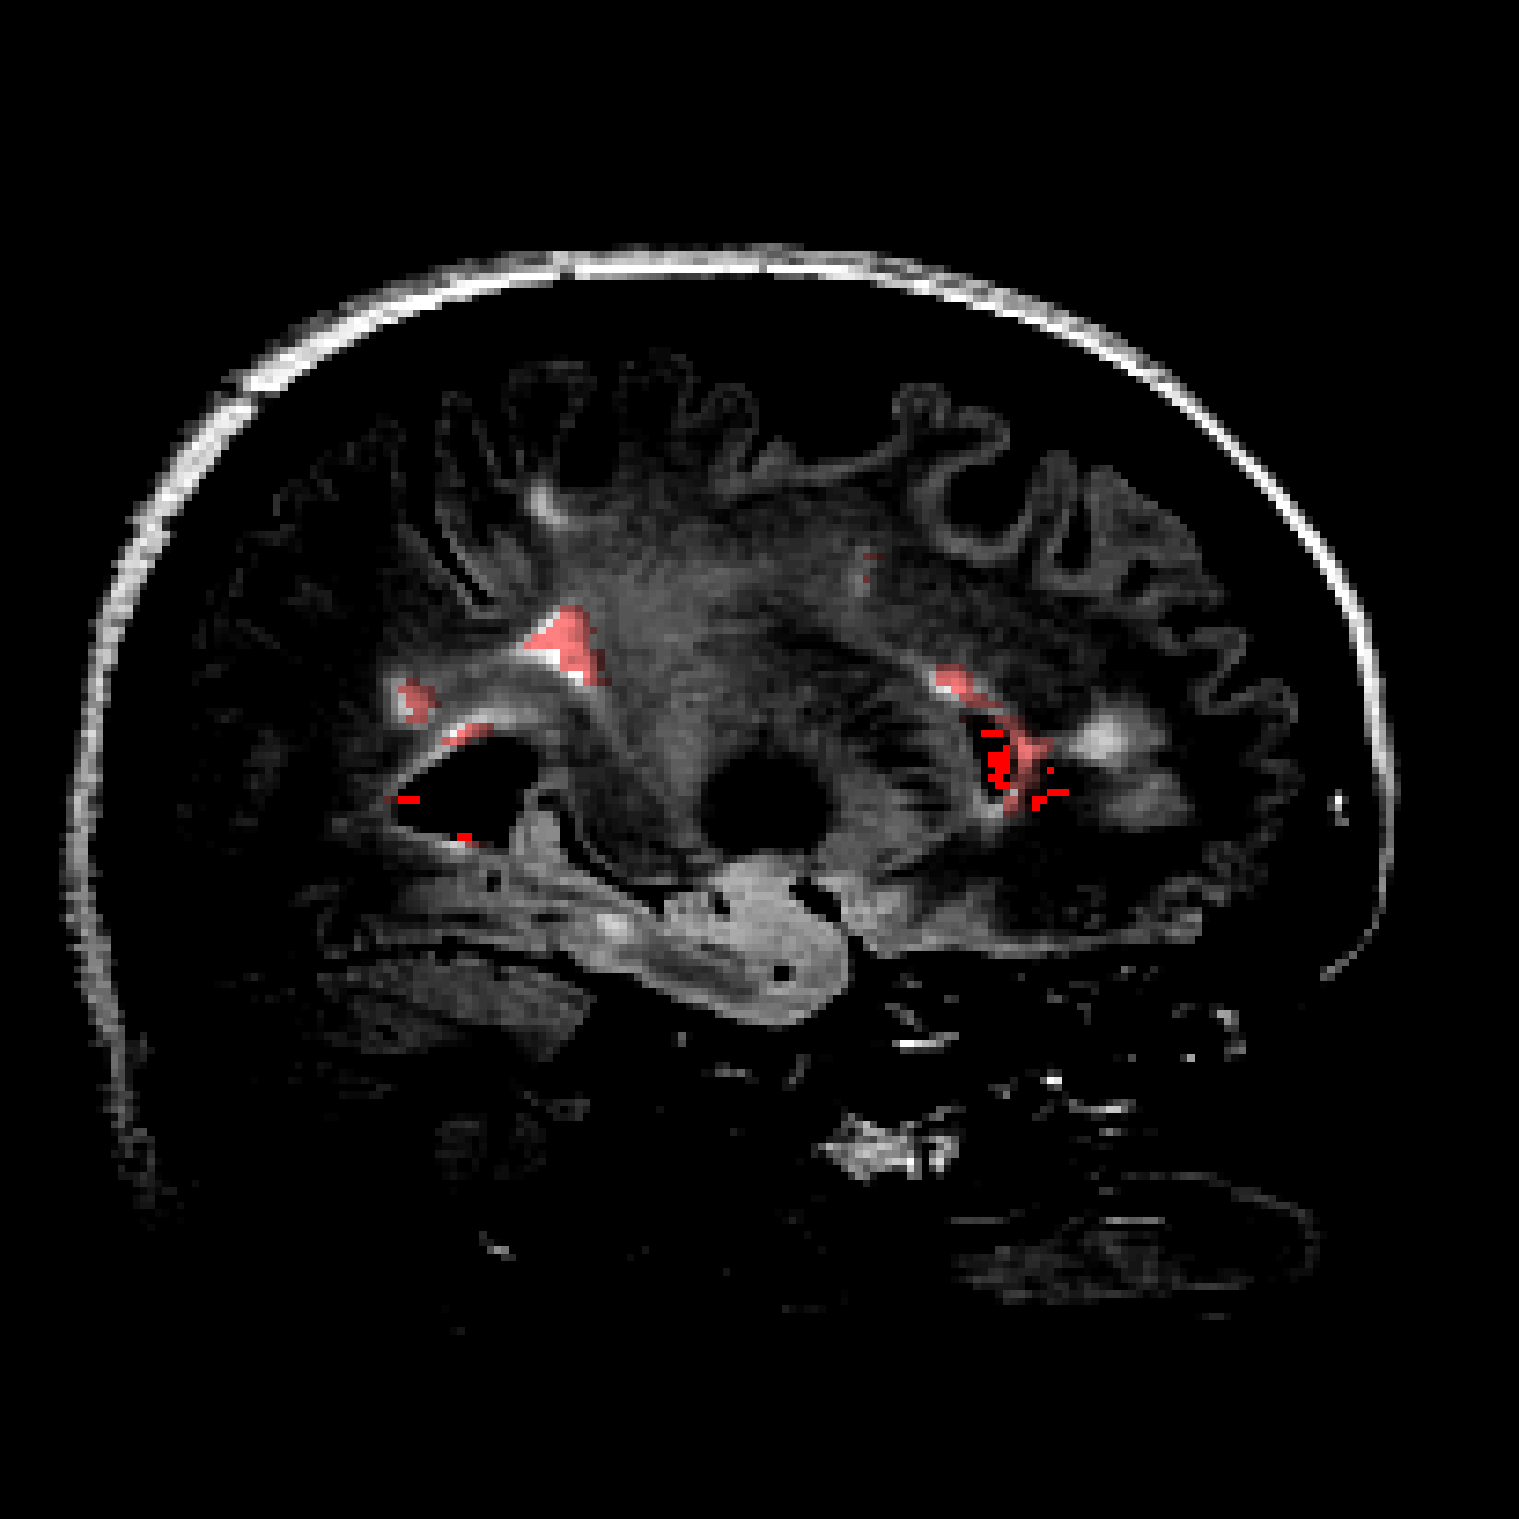
\includegraphics[height=6cm]{m08rev-05-d2-z107-o}\\[0.2em]
      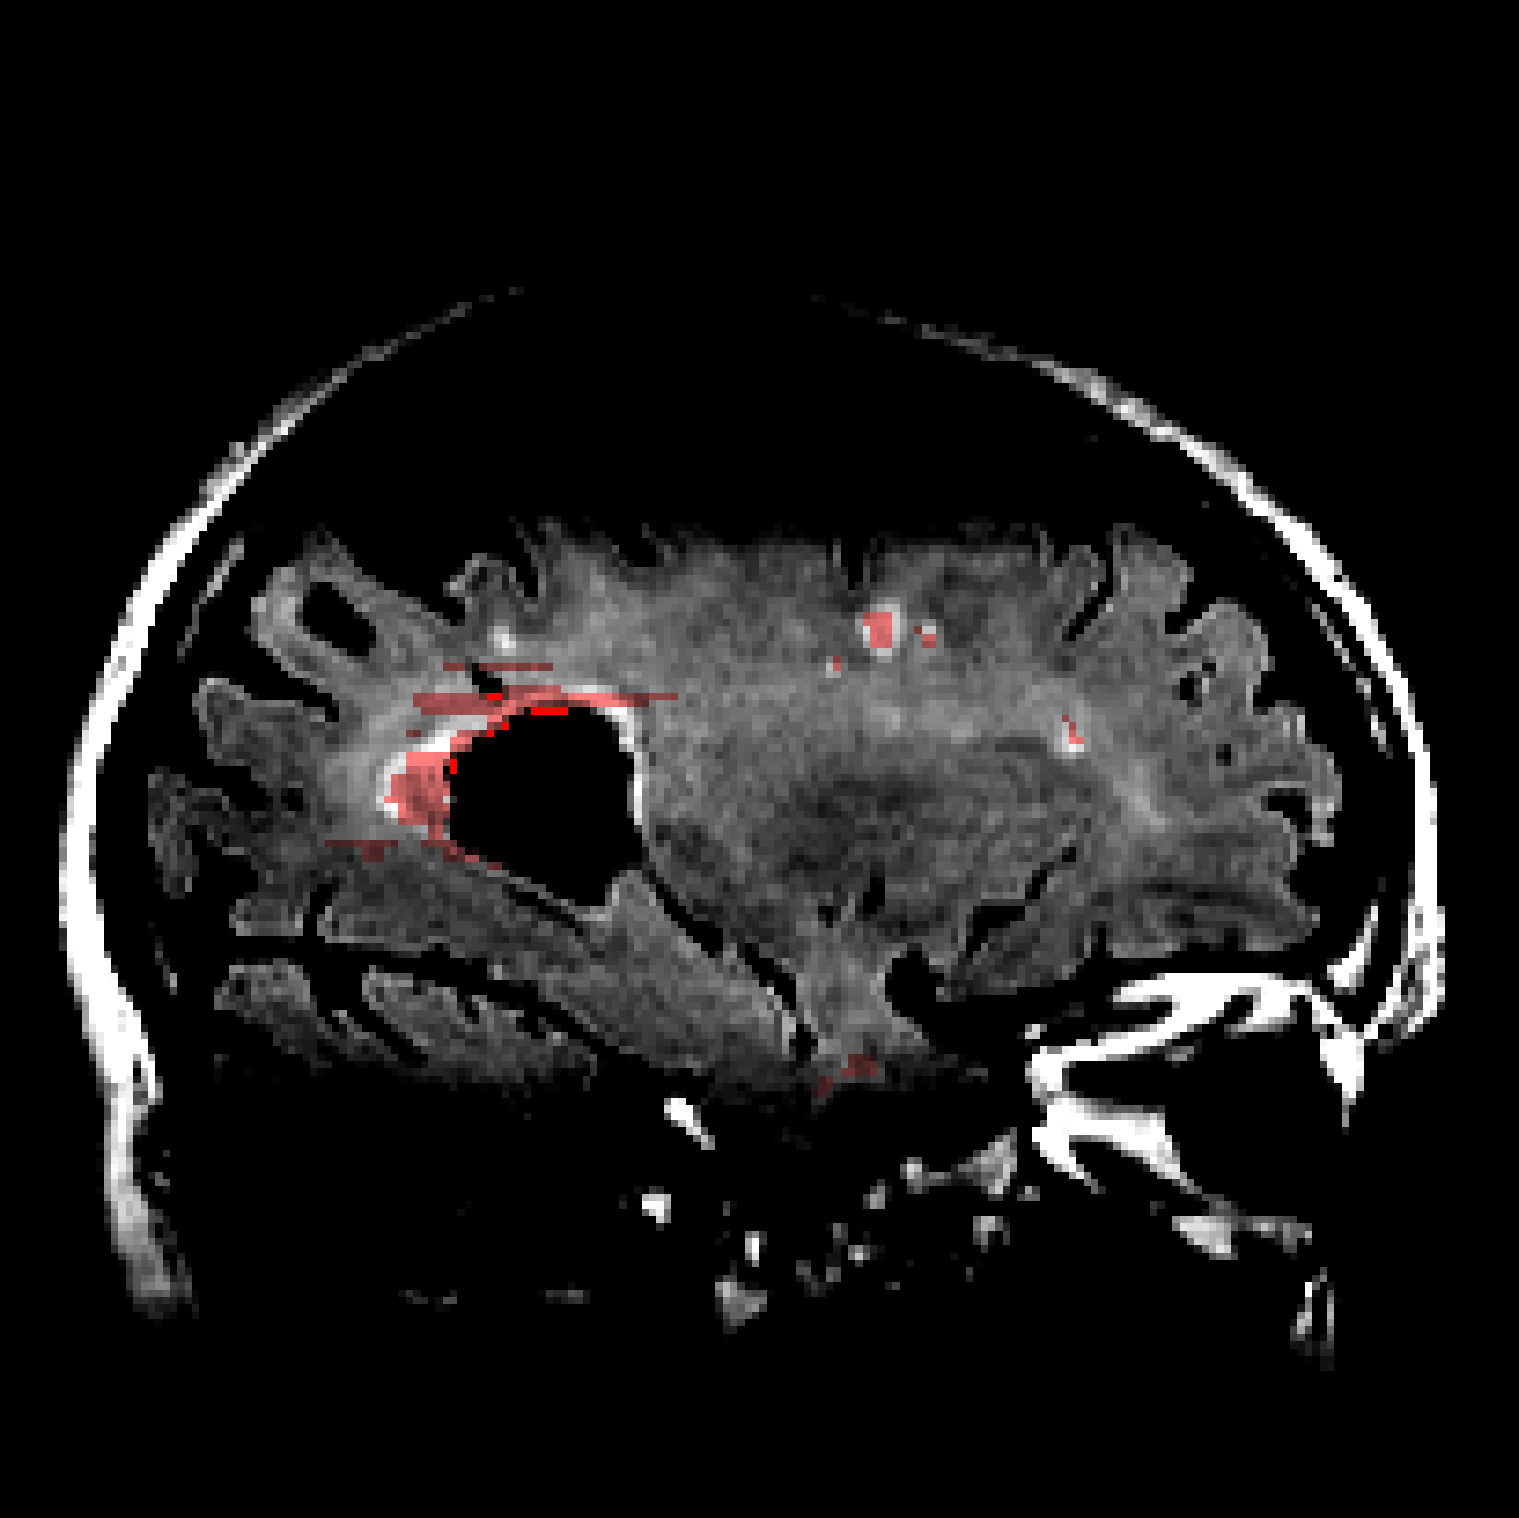
\includegraphics[height=6cm]{m08rev-06-d2-z101-o}
    \end{subfigure}
  \end{minipage}
  \begin{minipage}{6cm}
    \begin{subfigure}{\textwidth}
      \centering\subcaption{Revision}\label{fig:m08-rev-r}
      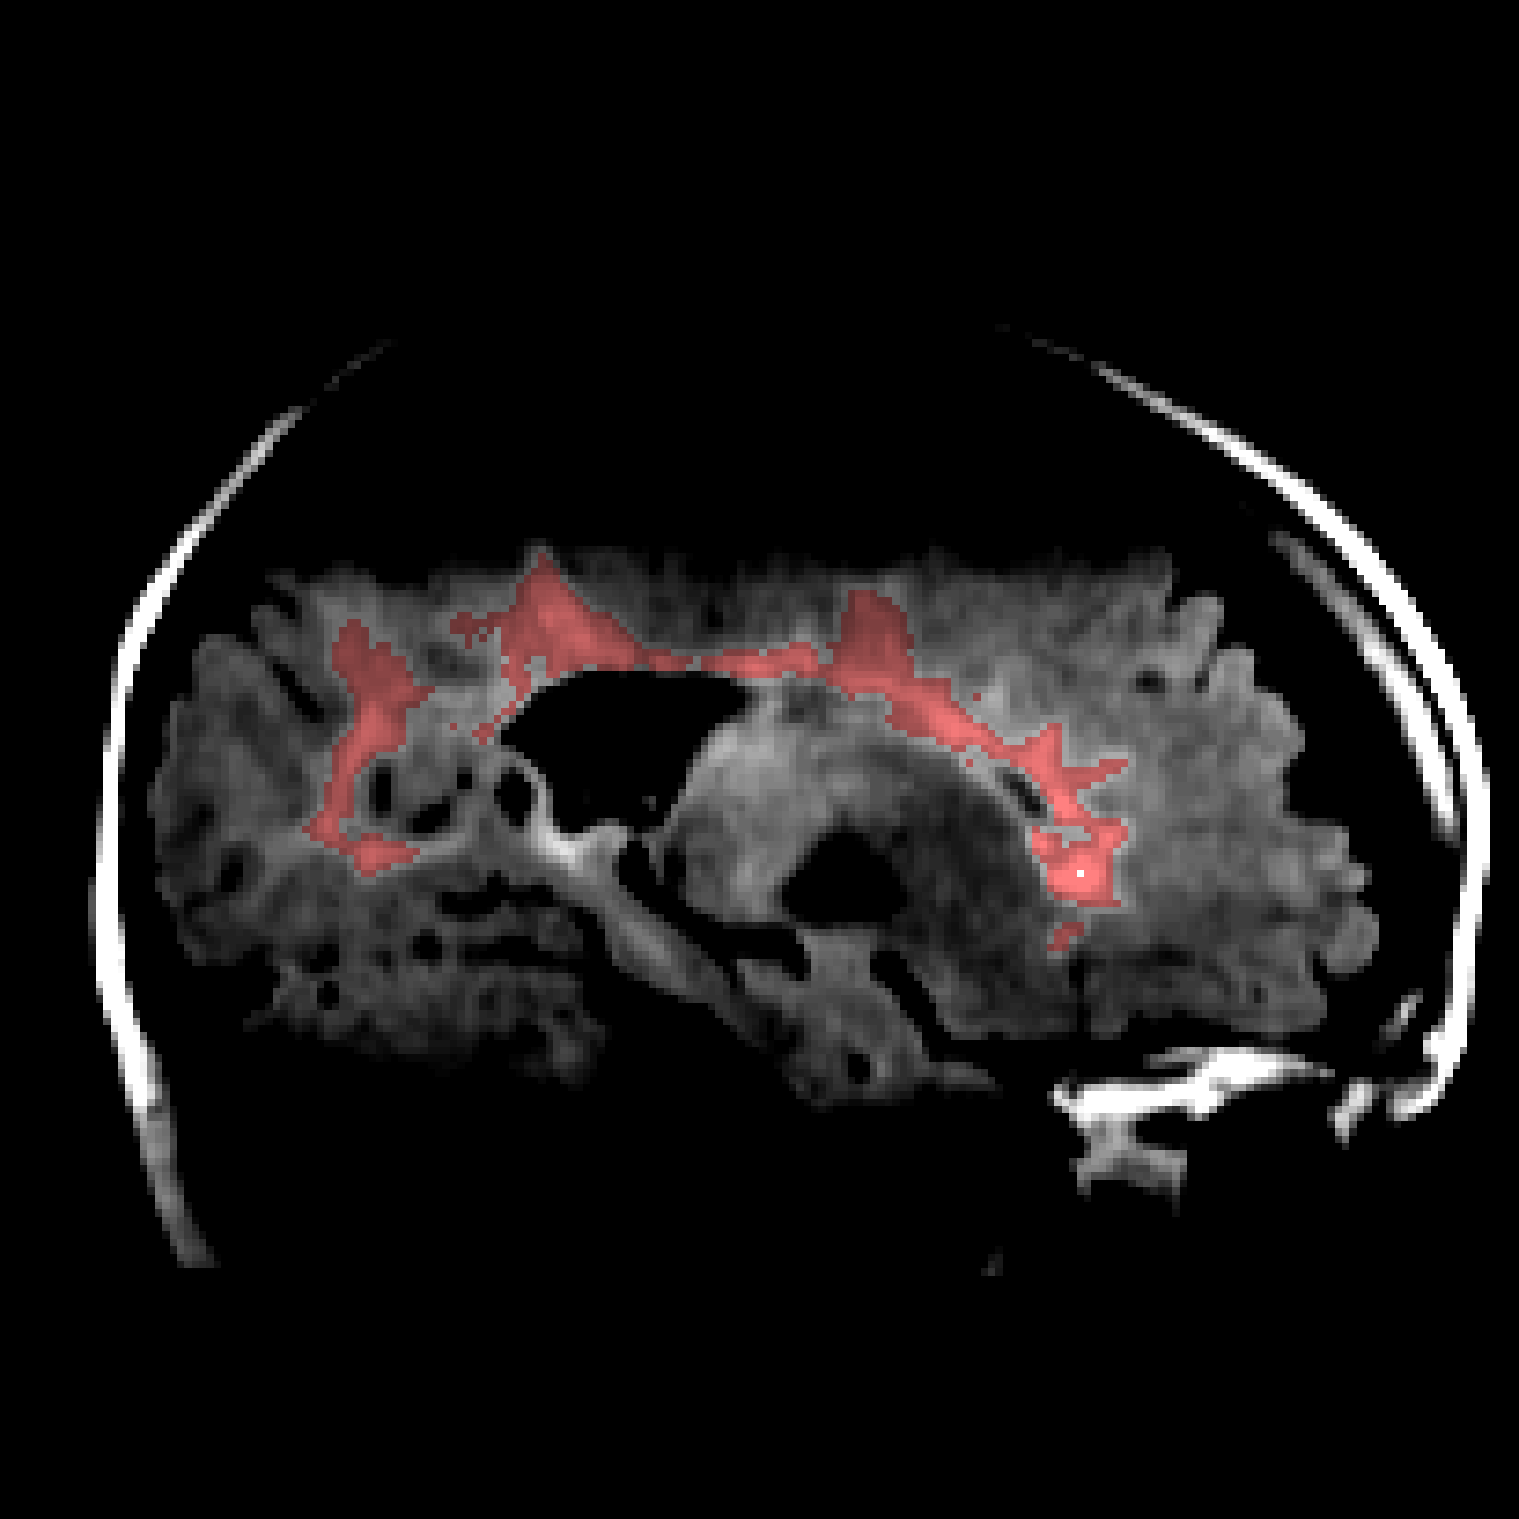
\includegraphics[height=6cm]{m08rev-01-d2-z146-r}\makebox[0pt][r]{\textcolor{white}{ CHB 01 }}\\[0.2em]
      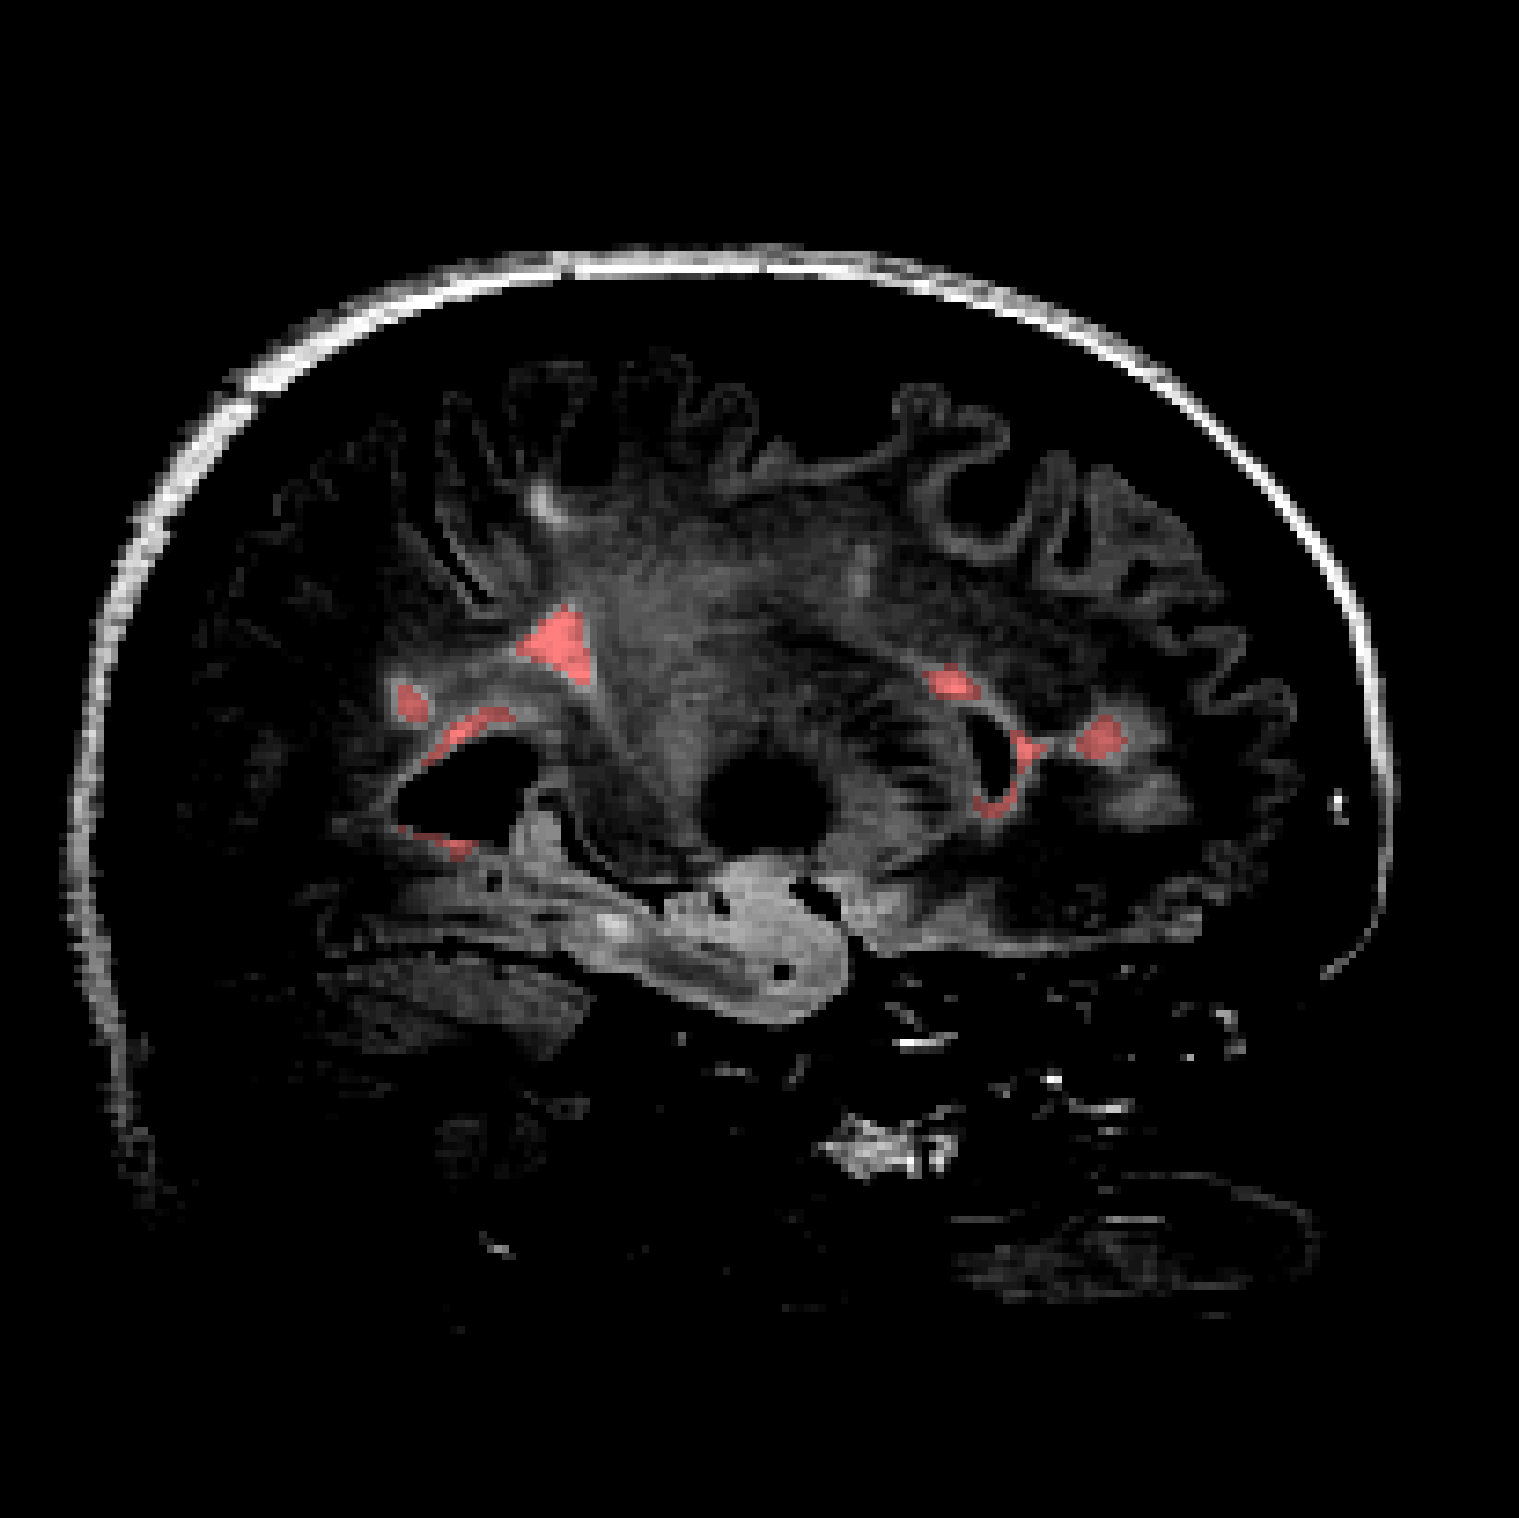
\includegraphics[height=6cm]{m08rev-05-d2-z107-r}\makebox[0pt][r]{\textcolor{white}{ CHB 05 }}\\[0.2em]
      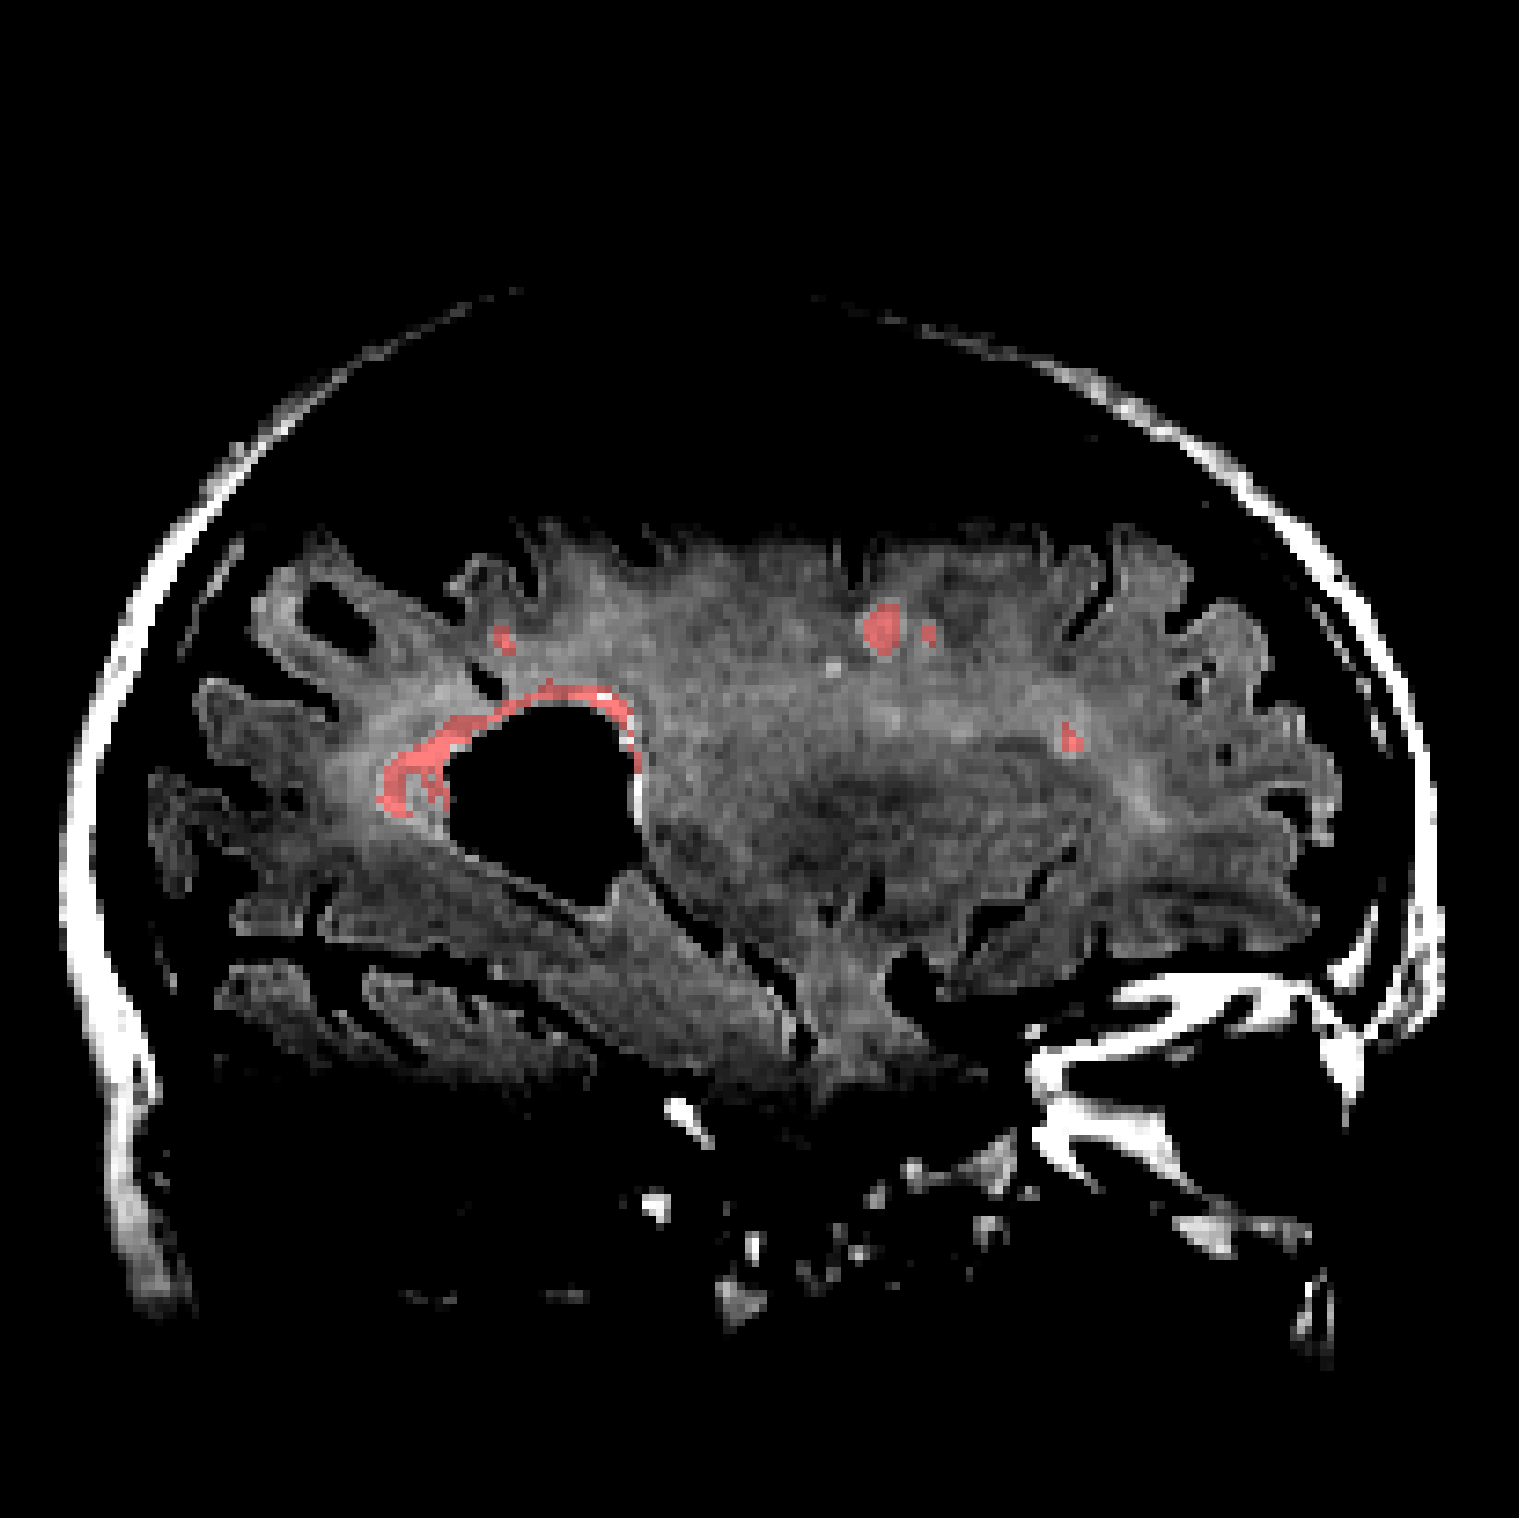
\includegraphics[height=6cm]{m08rev-06-d2-z101-r}\makebox[0pt][r]{\textcolor{white}{ CHB 06 }}
    \end{subfigure}
  \end{minipage}
  \caption{Example revisions to the manual segmentations for the MS 2008 challenge dataset.}
  \label{fig:m08-rev}
\end{figure}
% ==================================================================================================
\subsection{Brain Mask}\label{ss:brainmask}
In order to vectorize image data for parallel processing, a binary mask selecting voxels of interest in standardized space is also required. Since only voxels in the brain are of interest, this mask is called a ``brain mask''. The brain mask used here was derived from the ICBM tissue prior images \cite{Mazziotta2001} in MNI space: after initial thresholding of the combined $\gm+\wm+\csf$ probabilities at 0.5, manual refinements were completed and symmetry was enforced. The mask is slightly small on purpose, since tissues outside the brain are frequently bright in FLAIR images, and can be mistaken for lesions by naive models. The resulting mask is shown in Figure \ref{fig:brainmask}.
\begin{figure}
  \centering
  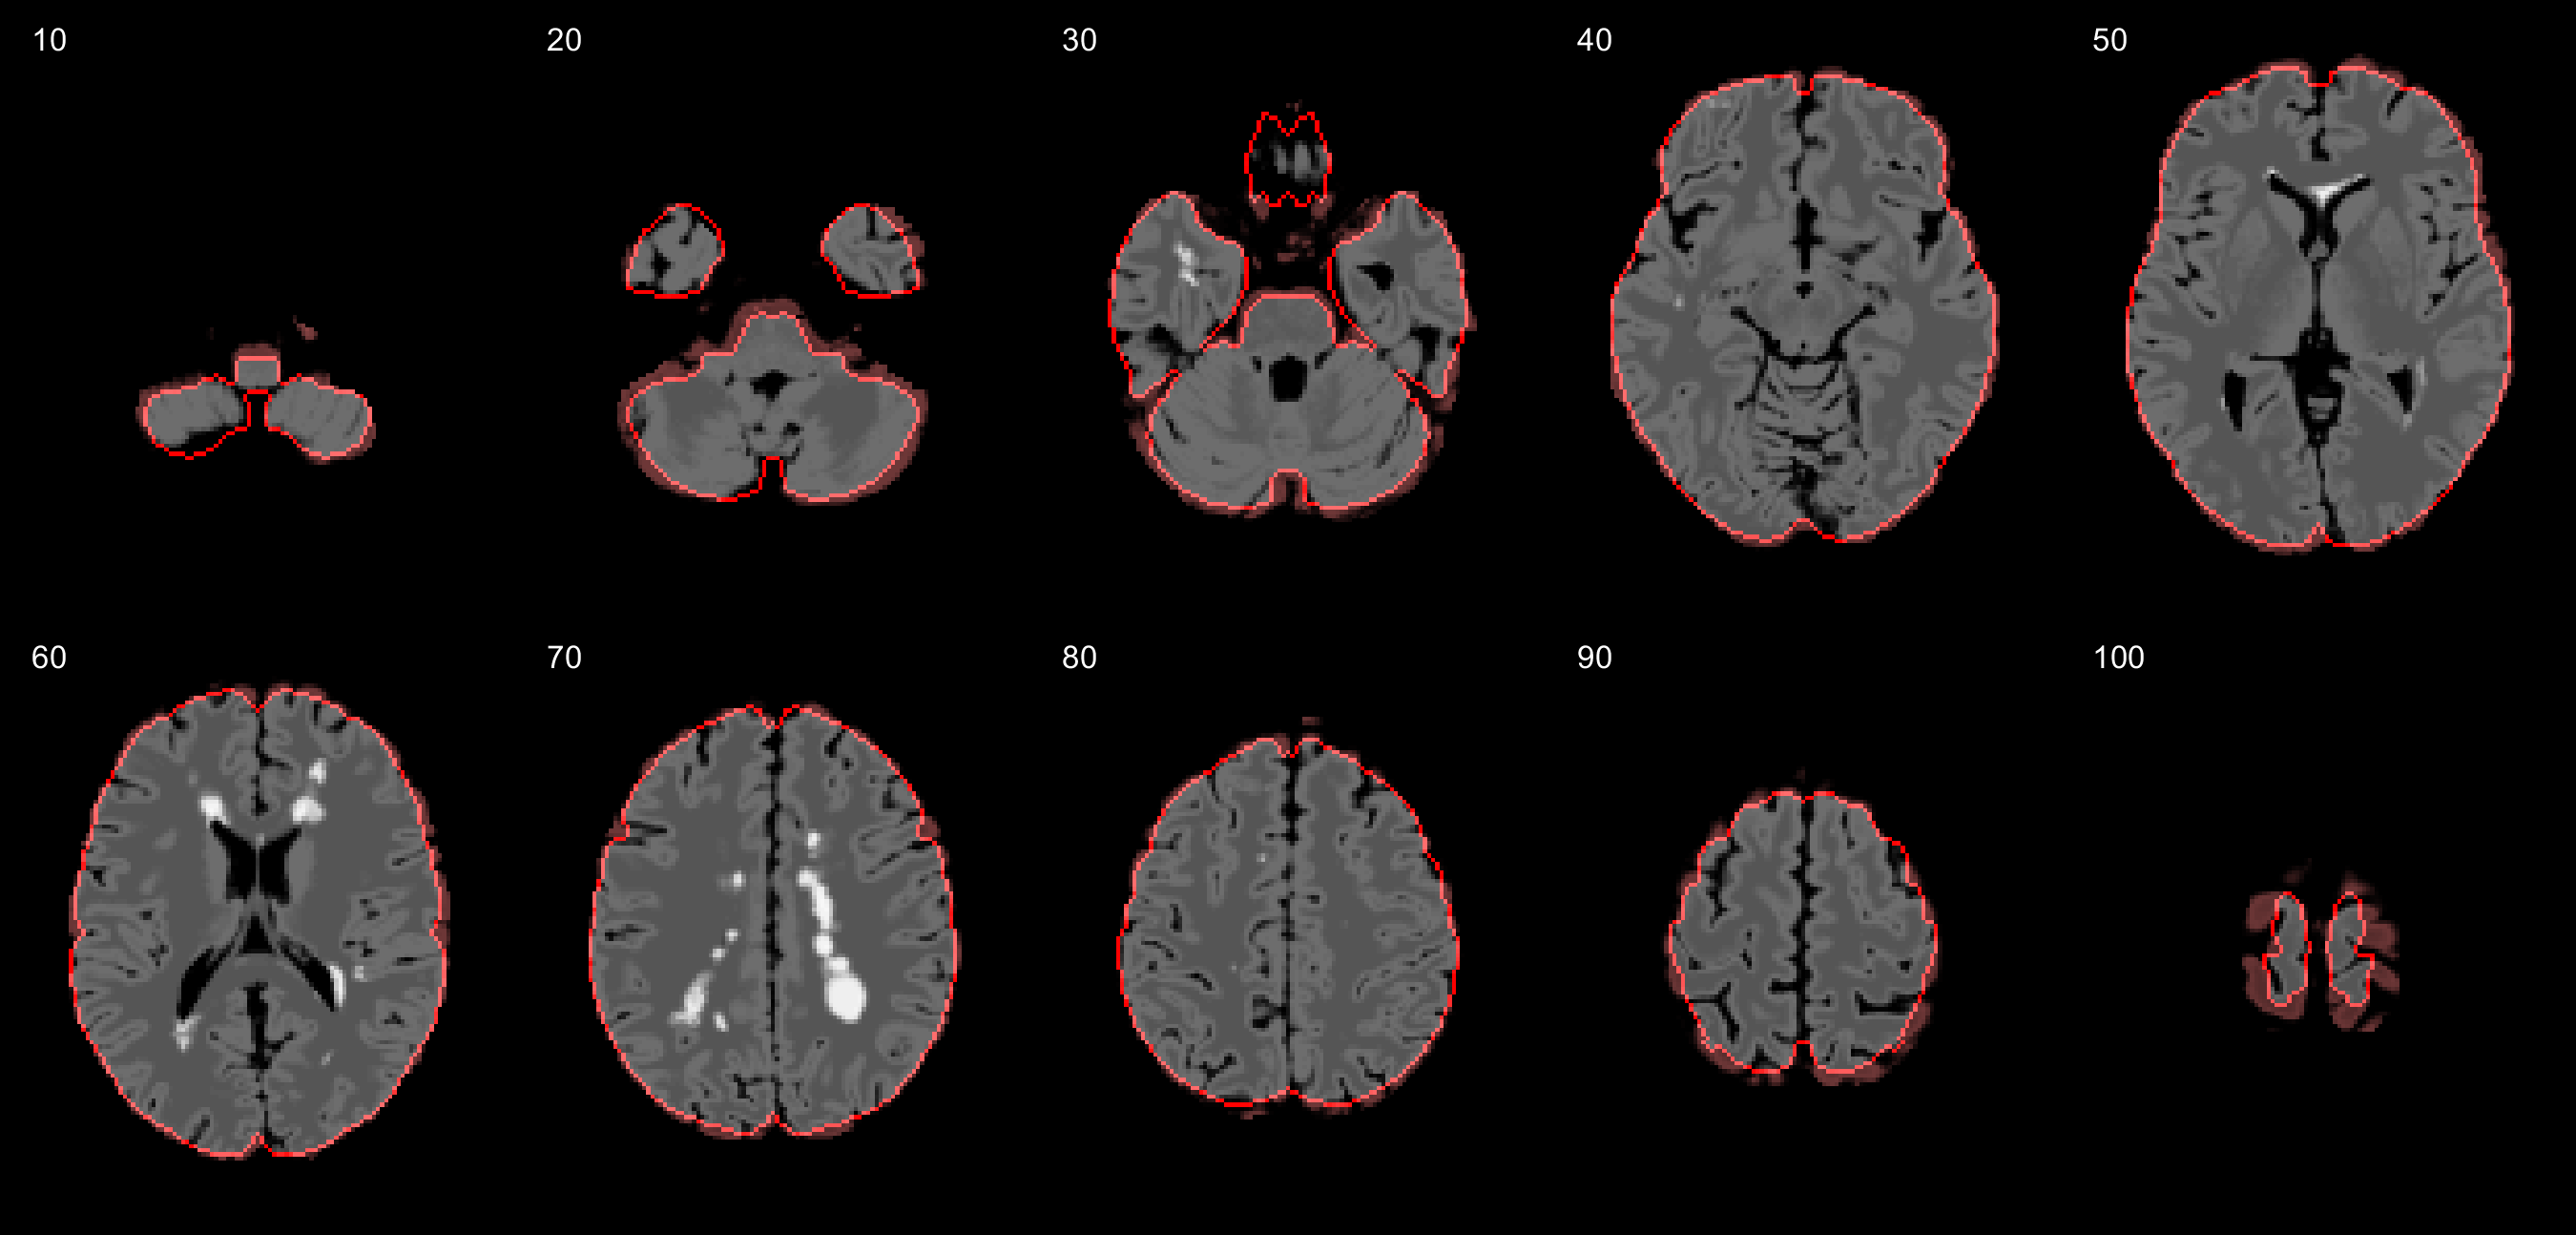
\includegraphics[height=2\sliceheight]{brainmask.png}
  \caption{Manually refined brain mask in MNI space. Mask outline is highlighted in red; inclusions are shown in grayscale; exclusions are tinted red.}
  \label{fig:brainmask}
\end{figure}
% --------------------------------------------------------------------------------------------------
% ==================================================================================================
%%%%%%%%%%%%%%%%%%%%%%%%%%%%%%%%%%%%%%%%%%%%%%%%%%%%%%%%%%%%%%%%%%%%%%%%%%%%%%%%%%%%%%%%%%%%%%%%%%%%
